\documentclass[a4paper,10pt]{article}

\usepackage{url,parskip}%formatting
\usepackage{titlesec}
\usepackage{supertabular}
\usepackage[utf8]{inputenc}
\usepackage{graphicx}
\usepackage{wrapfig}

\usepackage{hyperref}

\usepackage{fullpage}

\titleformat{\section}{\large\scshape\raggedright}{}{0em}{}[\titlerule]
\titlespacing{\section}{0pt}{0pt}{0pt}

\begin{document}
\pagestyle{empty}
  \begin{wrapfigure}{r}{0.25\textwidth}
  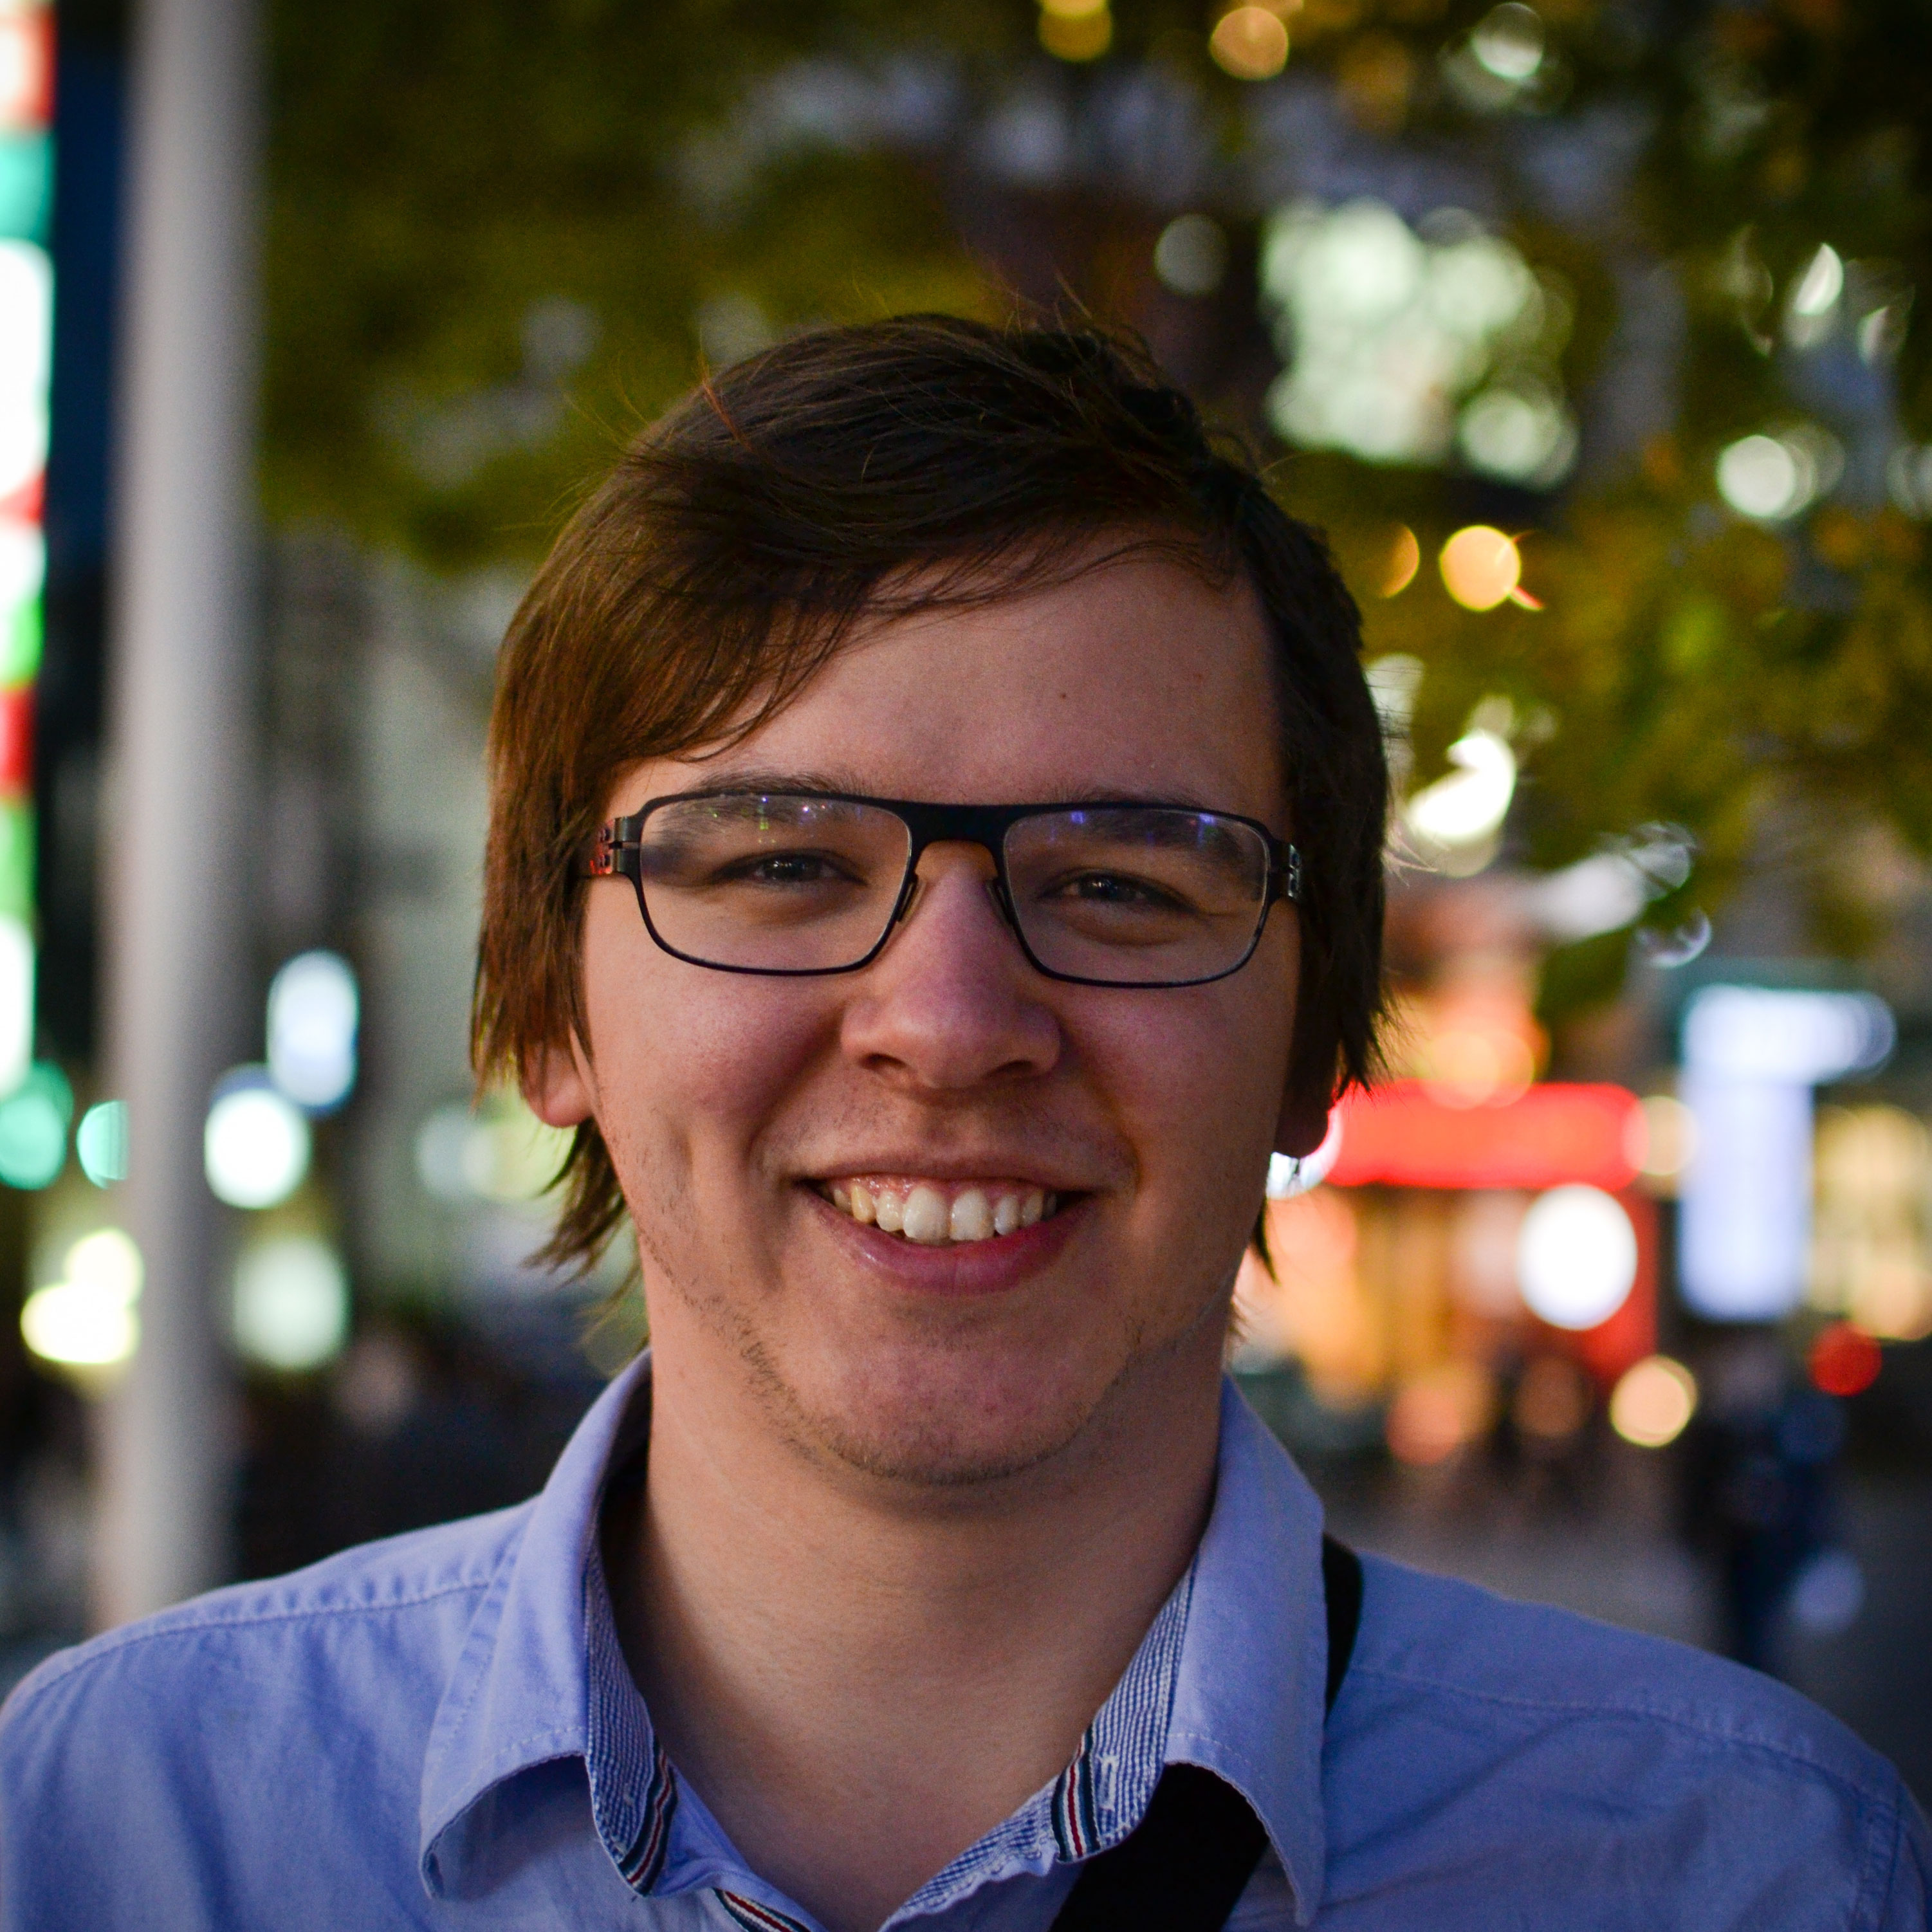
\includegraphics[width=0.25\textwidth]{profile.jpg}
  \end{wrapfigure}
% Title
\par{
  {\Huge Dag-Inge Aas }
  \bigskip\par}

% Personal Data
%  \section{Persona		l Data}
  \begin{tabular}{rl}
  \textsc{Date of Birth:} & 21 July 1989\\
    \textsc{Address:}& Schweigaards gate 63, 0656 Oslo\\
    \textsc{Phone:}& +47 924 91 526\\
    \textsc{Email:}& \href{mailto:daginge@confrere.com}{daginge@confrere.com}\\
    \textsc{Homepage:}& \href{http://daginge.com}{http://daginge.com}\\
    \textsc{Github:}& \href{http://github.com/dagingaa}{http://github.com/dagingaa}\\
\end{tabular}

\section{Summary}
\par{
Software Engineer with a passion for building tomorrows applications and services for the web. Likes to do large
scale system architecture and development. }

\section{Work Experience}
\begin{tabular}{r|p{12cm}}
  \emph{Current} & CTO \& Co-Founder at \textsc{Confrere}, Oslo \\\textsc{Jul 2017}&\
  \footnotesize{Confrere creates software to connect professionals with their clients over video. I co-founded this company together with Svein Willassen, and will be responsible for the technical aspects of the product. Stay tuned for more!}\\\multicolumn{2}{c}{} \\
  \textsc{Jan 2016} & Technical Lead at \textsc{appear.in}, Oslo \\\textsc{Jul 2017}&\
  \footnotesize{Had the main responsibility for the overall architecture and technical decisions for the appear.in premium product. Together with a team of engineers, we created a business oriented version of appear.in. I primarily worked on payment and billing, making sure we were compliant and easy to use. In addition, I onboarded engineers, held talks and workshops (both internally and externally at international conferences), managed business contacts and helped shape the product from idea to realization.}\\\multicolumn{2}{c}{} \\
  \textsc{Jun 2013} & Software Engineer at \textsc{appear.in}, Oslo  \\\textsc{Jul 2017}&\
  \footnotesize{Created appear.in, video conferencing for teams as it was meant to be. Worked on pretty much everything. I've had my hands in the backend (Node.js), frontend (Angular.js/React) and Android. I also participated actively in product development, marketing, feature prioritisation, and more.}\\\multicolumn{2}{c}{} \\
  \textsc{Jan 2012} & Software Engineer Intern at \textsc{Telenor Digital}, Oslo  \\\textsc{Jun 2013}&\
  \footnotesize{Software developer. Has worked on scalable end-to-end browser testing in the cloud. Also created both the engineering blog and careers page using Jekyll on GitHub Pages. Created prototypes for new services using AngularJS, Node.JS, Grunt and Yeoman. Was a full time hire summer 2013 designing and building an OAuth implementation in Java using Jetty and Jersey. The component has since become a vital part of the backend infrastructure in Telenor Digital, powering authentication and authorization on most of our services.}\\\multicolumn{2}{c}{} \\
\end{tabular}

\section{Education}
\begin{tabular}{r|p{12cm}}
  \textsc{Jun 2013} & \textsc{Norwegian University of Science and Technology} \\\textsc{Aug 2008}&\emph{Master of Science in Computer Science}\\&\footnotesize{Specialized in Software and Information Systems.} \\& \footnotesize{Notable courses: Object-oriented Programming, Algorithms and Data structures, Information Systems, Programming Languages, Software Architecture, Software Quality and Quality Assurance, Software Security, Distributed Systems, Project Management.}\\\multicolumn{2}{c}{} \\
\end{tabular}

\section{Volunteer work}
\begin{tabular}{r|p{12cm}}
  \emph{Current} & Head of IT at ISFiT 2013, Trondheim  \\\textsc{Aug 2011}&\emph{Head of Development and System Administration}\\&\footnotesize{The Head of IT is responsible for the entire infrastructure of ISFiT. This includes development, maintenance and system administration for a festival with over 400 volunteers. ISFiT has 5 major IT projects, ranging from editorial tools to system administration. I oversee the development and maintenance of these five projects, with 8 developers actively working on them. I also participate in board meetings in the information section, creating and spreading ISFiT 2013 to the world. See also "Head of Development"}\\\multicolumn{2}{c}{} \\
  \emph{Aug 2011} & Head of Development at ISFiT 2011, Trondheim  \\\textsc{Mar 2010}&\emph{Ruby on Rails Developer and Project Manager}\\&\footnotesize{Project manager for the biggest new IT project of ISFiT 2011. Held meetings, workshops and demonstrations, gathered requirement specification from the different affected parties and maintaned the project after launch. Led a group of 3 other developers from start to finish to maintenance. Programming was mainly focused on Ruby on Rails and scripting using Ruby. Some of our core technologies include LDAP, MySQL, UNIX, Apache, Passenger, capistrano and more.}\\\multicolumn{2}{c}{} \\
\end{tabular}

\section{Skills}
\begin{tabular}{r|p{12cm}}
  \textsc{Technical}& Programming languages  \\&\footnotesize{JavaScript, Java, Ruby and Python. In addition I have experience building distributed systems on Amazon Web Services handling millions of users, as well as architecture for large web applications in AngularJS and React. }
  \\\multicolumn{2}{c}{}\\

\end{tabular}


\end{document}
